\section{State Estimation}
\subsection{Estimation State-matrices}

%% State Space Model
Using equation (6a-6c) we derived the following matrices for the state space model

% $$
%     \ddot{\widetilde{p}} = K_1 \tilde{V_d} %\xrightarrow{\int}K_1 \tilde{V_d} t %\xrightarrow{\int} \frac{1}{2} K_1 %\tilde{V_d} t^2 = \widetilde{p}
% $$

% $$
%     \ddot{\widetilde{e}} = K_2 %\tilde{V_s}\xrightarrow{\int}K_2 \tilde{V_s} %t\xrightarrow{\int} \frac{1}{2} K_1 %\widetilde{V_s} t^2 = \widetilde{e}
% $$
% $
% \ddot{\widetilde{\lambda}} = K_3 %\widetilde{p}\xrightarrow{\int}K_3 %\widetilde{p} t\xrightarrow{\int} \frac{1}{2} %K_3 \widetilde{p} t^2 = \widetilde{e}
% $$

\begin{align}
    A = \begin{bmatrix}0&1&0&0&0&0\\0&0&0&0&0&0\\0&0&0&1&0&0\\0&0&0&0&0&0\\0&0&0&0&0&1\\ K_3&0&0&0&0&0 \end{bmatrix} 
    \quad   
    B = \begin{bmatrix} 0&0\\0&K_1\\0&0\\K_2&0\\0&0\\0&0 \end{bmatrix} 
    \quad 
    C = \begin{bmatrix} 1&0&0&0&0&0 \\ 0&0&1&0&0&0 \\ 0&0&0&0&1&0 \end{bmatrix}
\end{align}

with state vectors

\begin{align}
    x = \begin{bmatrix}
        \tilde{p}\\
        \dot{\tilde{p}}\\
        \tilde{e}\\
        \dot{\widetilde{e}}\\
        \tilde{\lambda}\\
        \dot{\tilde{\lambda}} 
        \end{bmatrix}, \quad
    u = \begin{bmatrix}
        \tilde{V_s}\\
        \tilde{V_d} 
        \end{bmatrix}, \quad
    y = \begin{bmatrix}    
        \tilde{p}\\
        \tilde{e}\\
        \tilde{\lambda} 
        \end{bmatrix}
\end{align}


%%Observability Mat

\subsection{Observability and State Observer}
In order to examine the state observer we calculated the observability matrix, which is given by
\begin{equation*}
    \mathcal{O} = 
    %\fixTABheight{}
    \bracketMatrixstack{
        C\\CA\\\vdots{}\\CA^5    
    }
\end{equation*}

which has $ rank = n = 6 $, thus the system is observable.\\
The linear observer used is given by
%
\begin{equation*}
    \dot{\vec{x}} = \vec{A\hat{x}} + \vec{Bu} + \vec{L}(\vec{Y} - \vec{C\hat{x}})
\end{equation*}
%
where $\vec{L}$ is the observer gain matrix. 
To calculate $\vec{L}$ we first looked at the eigenvalues of our system $(\vec{A}-\vec{BK})$, then adjusting the poles such that the estimator becomes 10-100 faster. $\vec{L}$ was calculated by using the MATLAB-command
%
\begin{lstlisting}  
    L = place(A', B', poles)';
\end{lstlisting}
%
The poles were placed on a circle with radius 40 in the complex plane (\cref{fig:poles}). This resulted in fast control without the noise affecting the system too much. Choosing a smaller radius made the estimator too slow, while increasing the radius too much led to a very noisy signal, as shown in figure \cref{fig:plot1} and \cref{fig:plot2}


\begin{figure}[H]
    \centering
    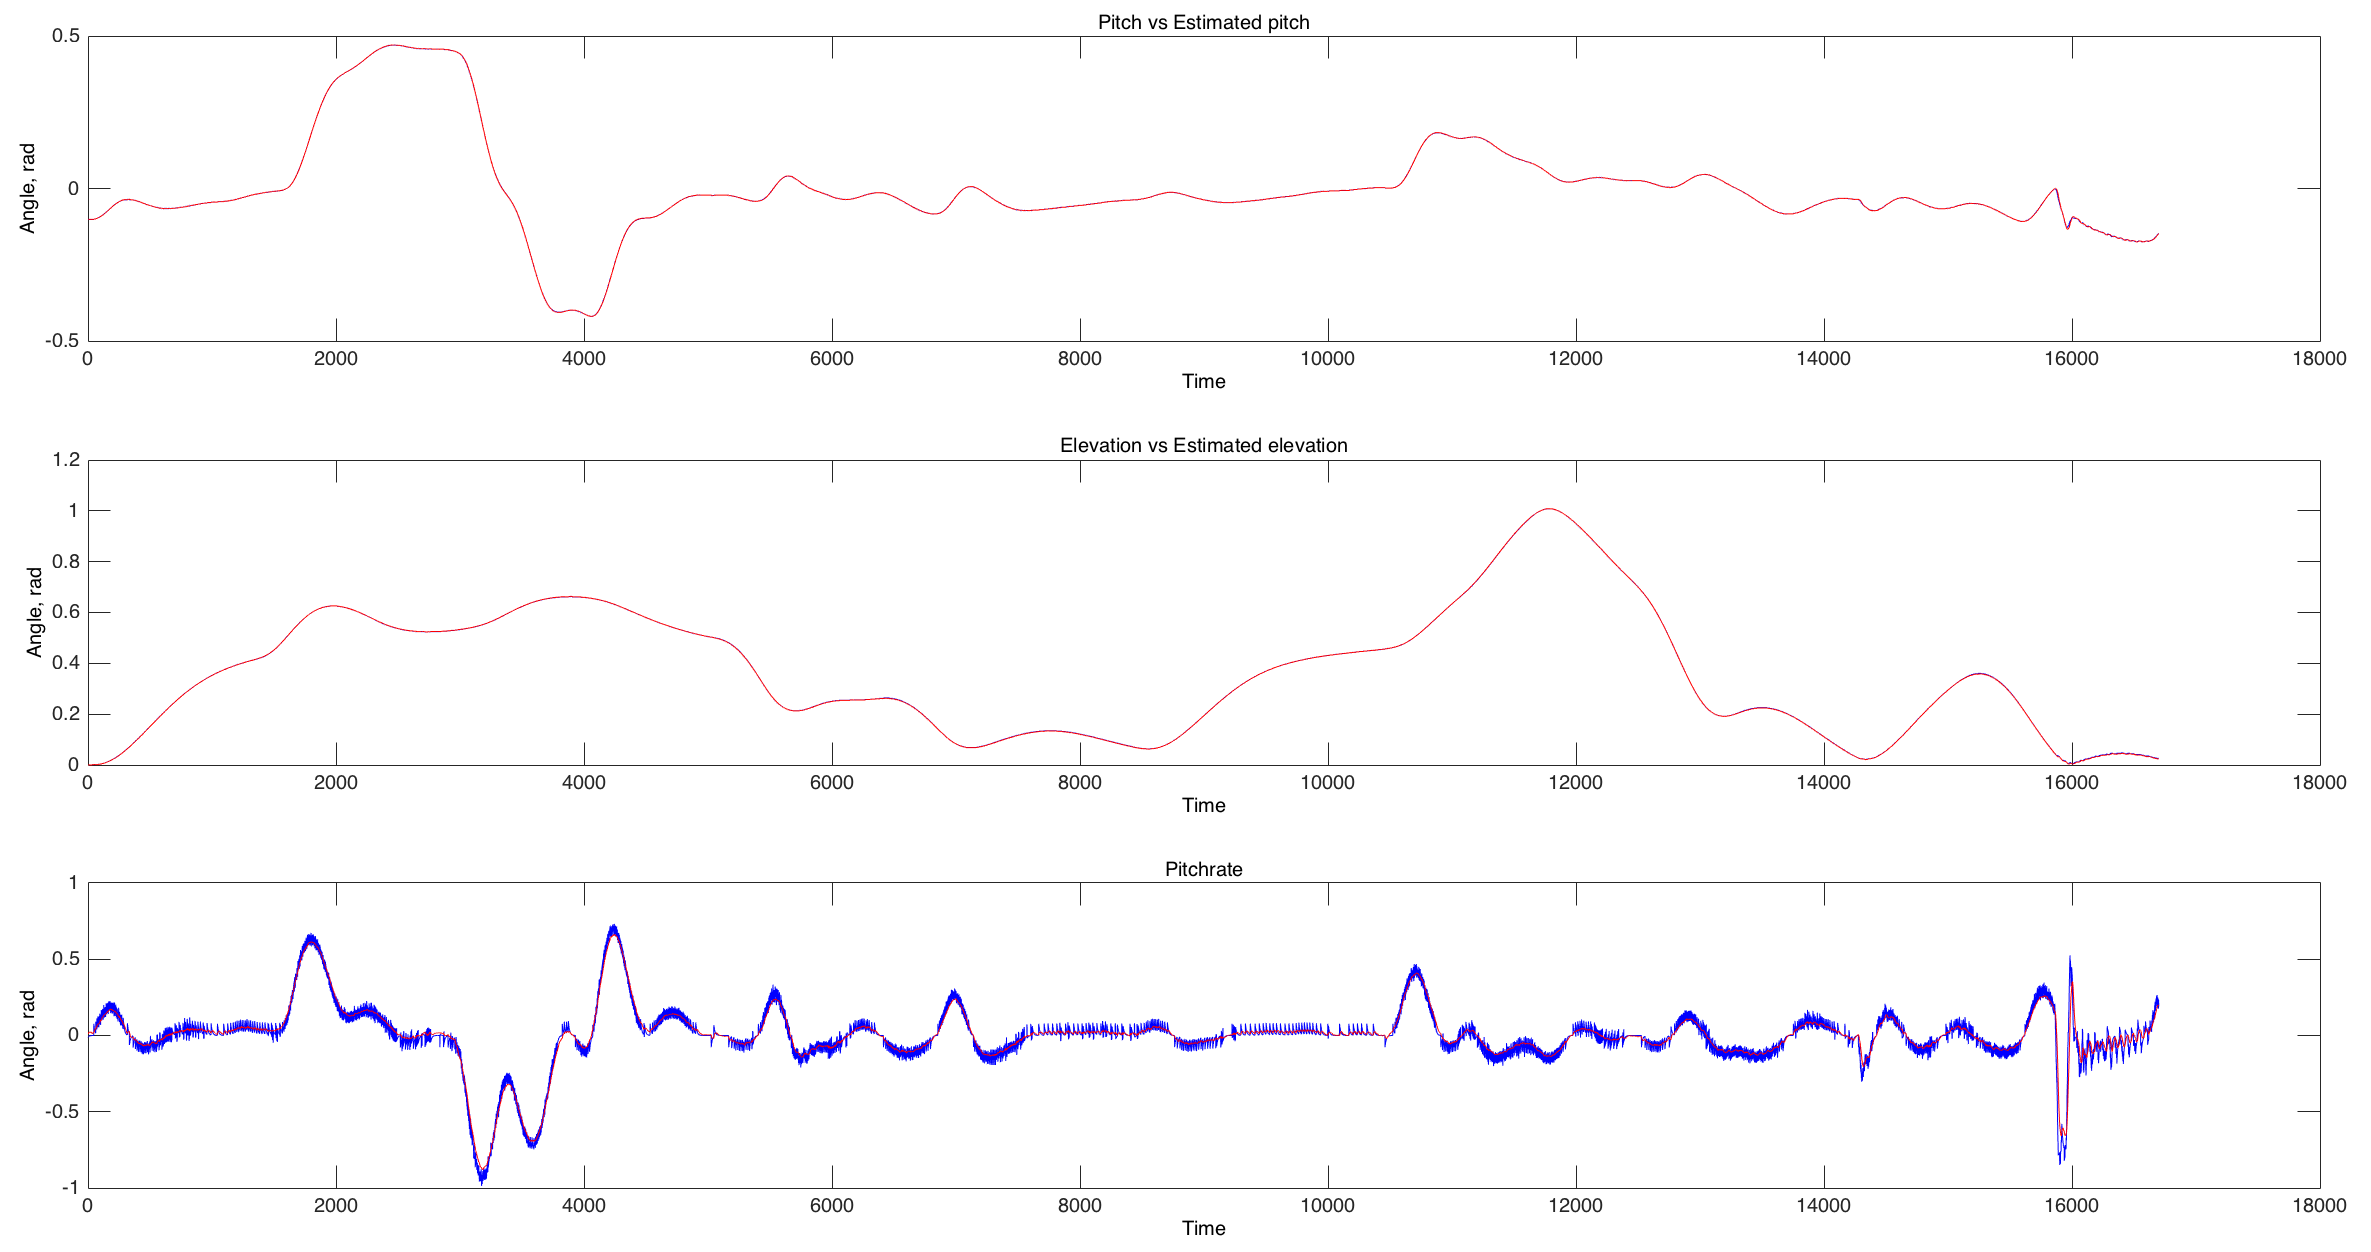
\includegraphics[width=1.0\textwidth]{pitchNpitchrate_P.png}
    \caption{Comparison of measured and estimated values of pitch, elevation and pitch rate in the P-controller (\emph{\color{blue}Blue} = measured value, \emph{\color{red} red} = estimated value)}
    \label{fig:plot1}
\end{figure}

\begin{figure}[H]
    \centering
    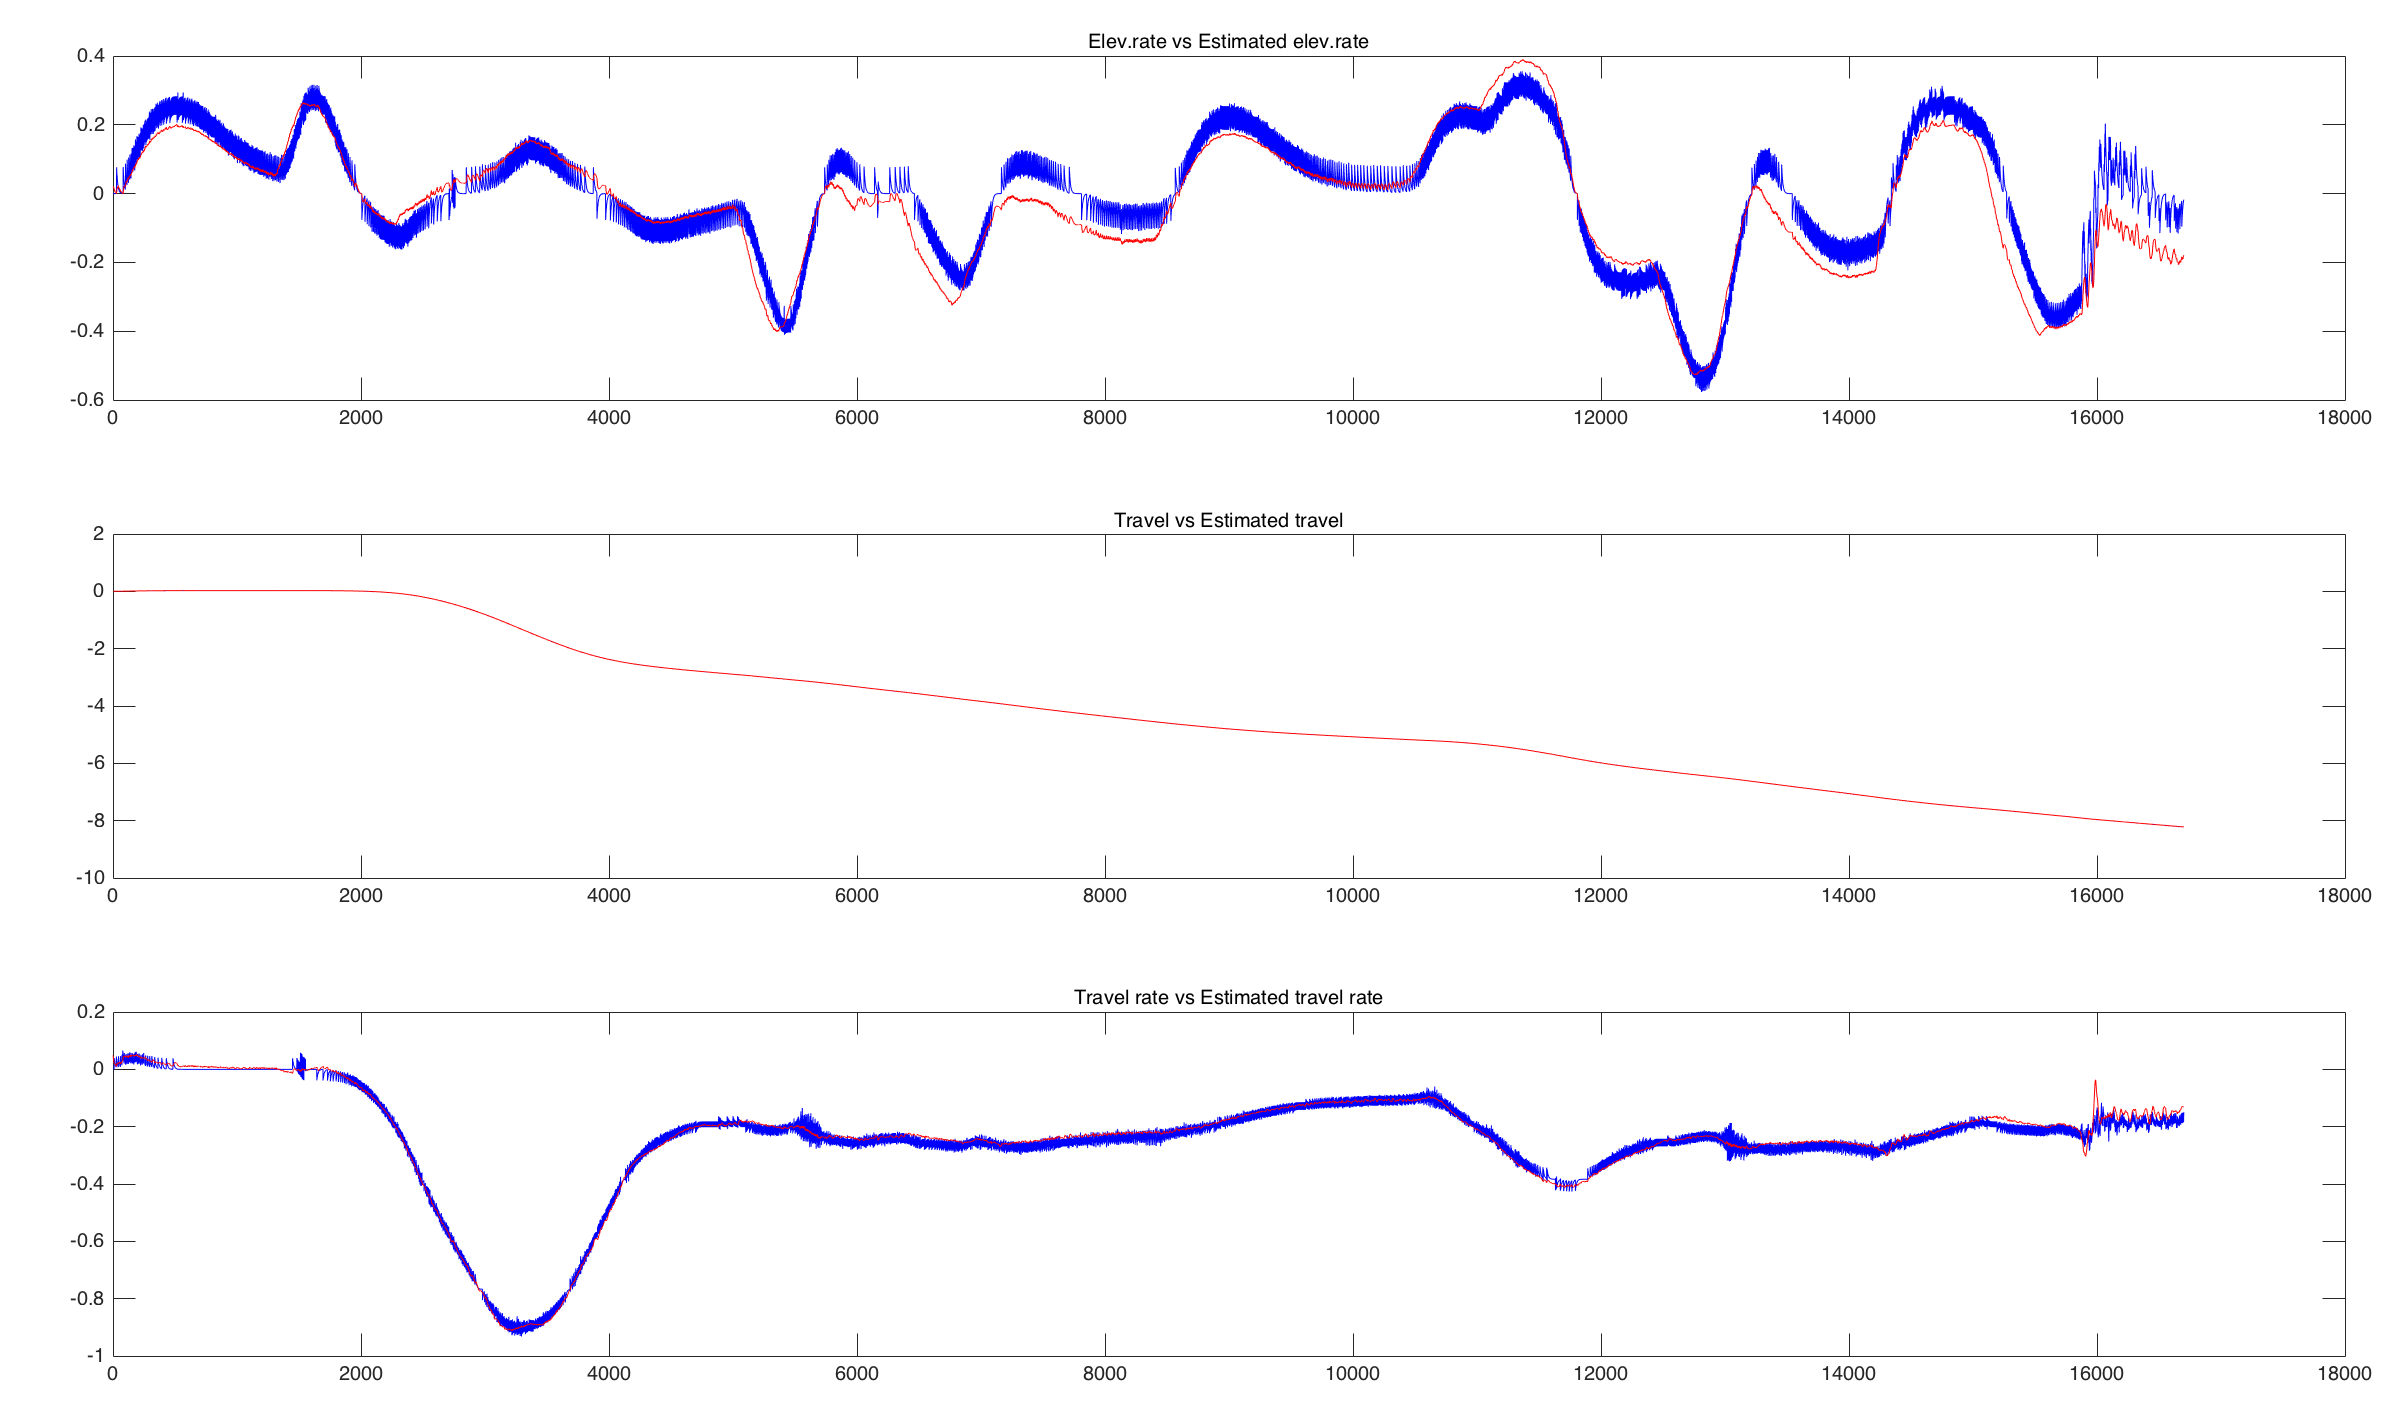
\includegraphics[width=1.0\textwidth]{elevrateP.png}
    \caption{Comparison of measured and estimated values of elevation rate, travel and travel rate in the P-controller (\emph{\color{blue}Blue} = measured value, \emph{\color{red} red} = estimated value)}
    \label{fig:plot2}
\end{figure}

\begin{figure}[H]
    \centering
    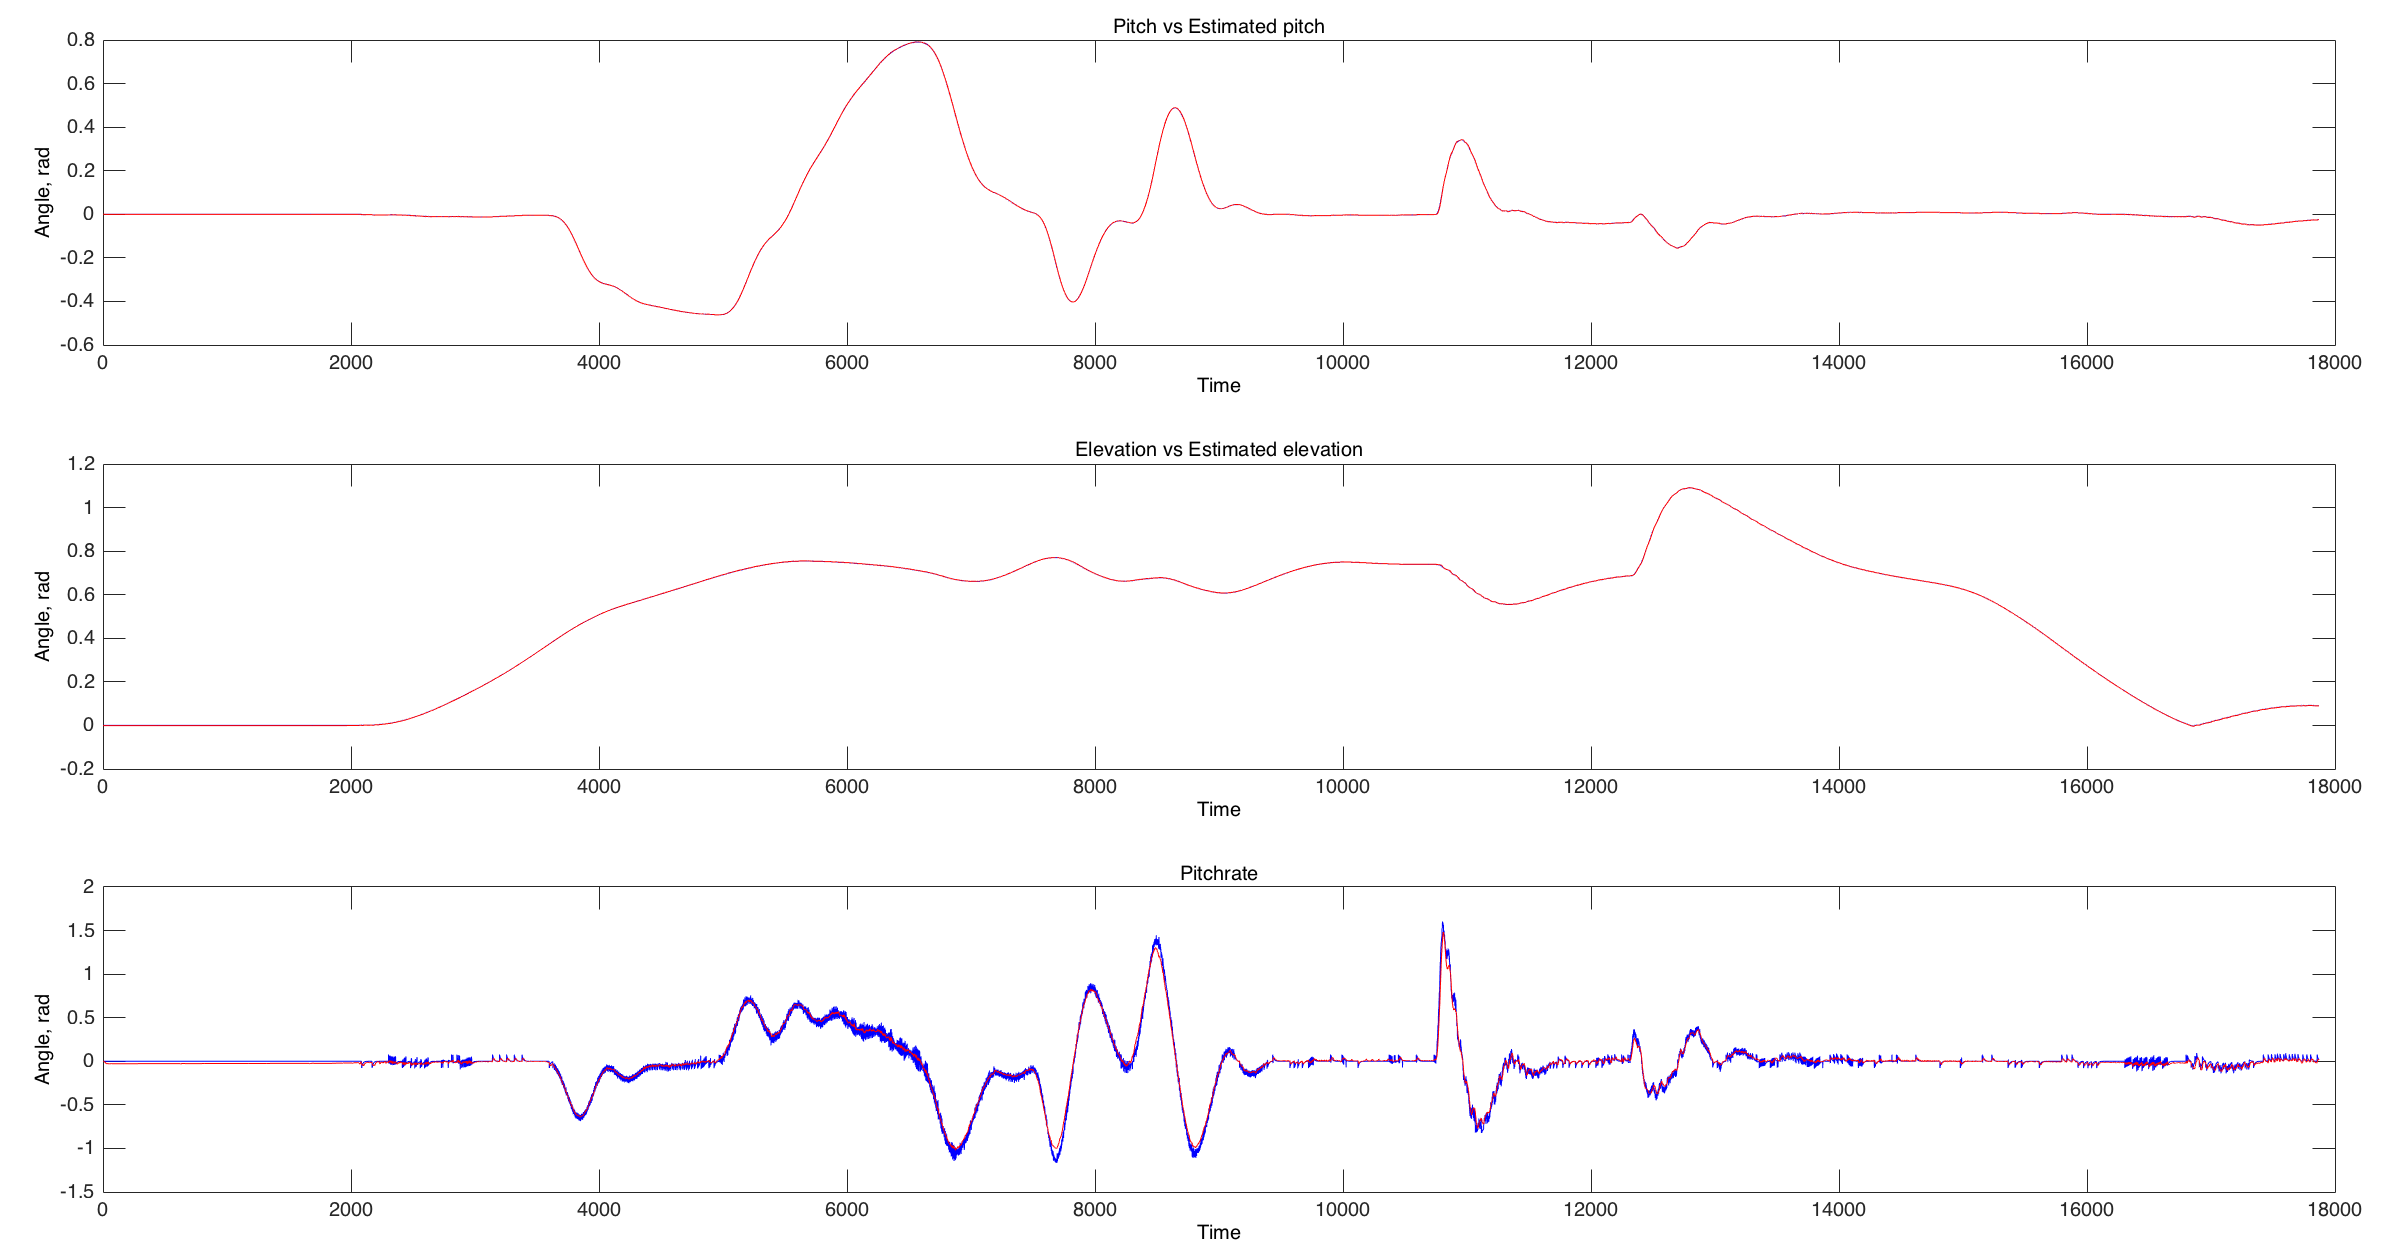
\includegraphics[width=1.0\textwidth]{pitchrate_PI.png}
    \caption{Comparison of measured and estimated values of pitch, elevation and pitch rate in the PI-controller (\emph{\color{blue}Blue} = measured value, \emph{\color{red} red} = estimated value)}
    \label{fig:plot3}
\end{figure}

\begin{figure}[H]
    \centering
    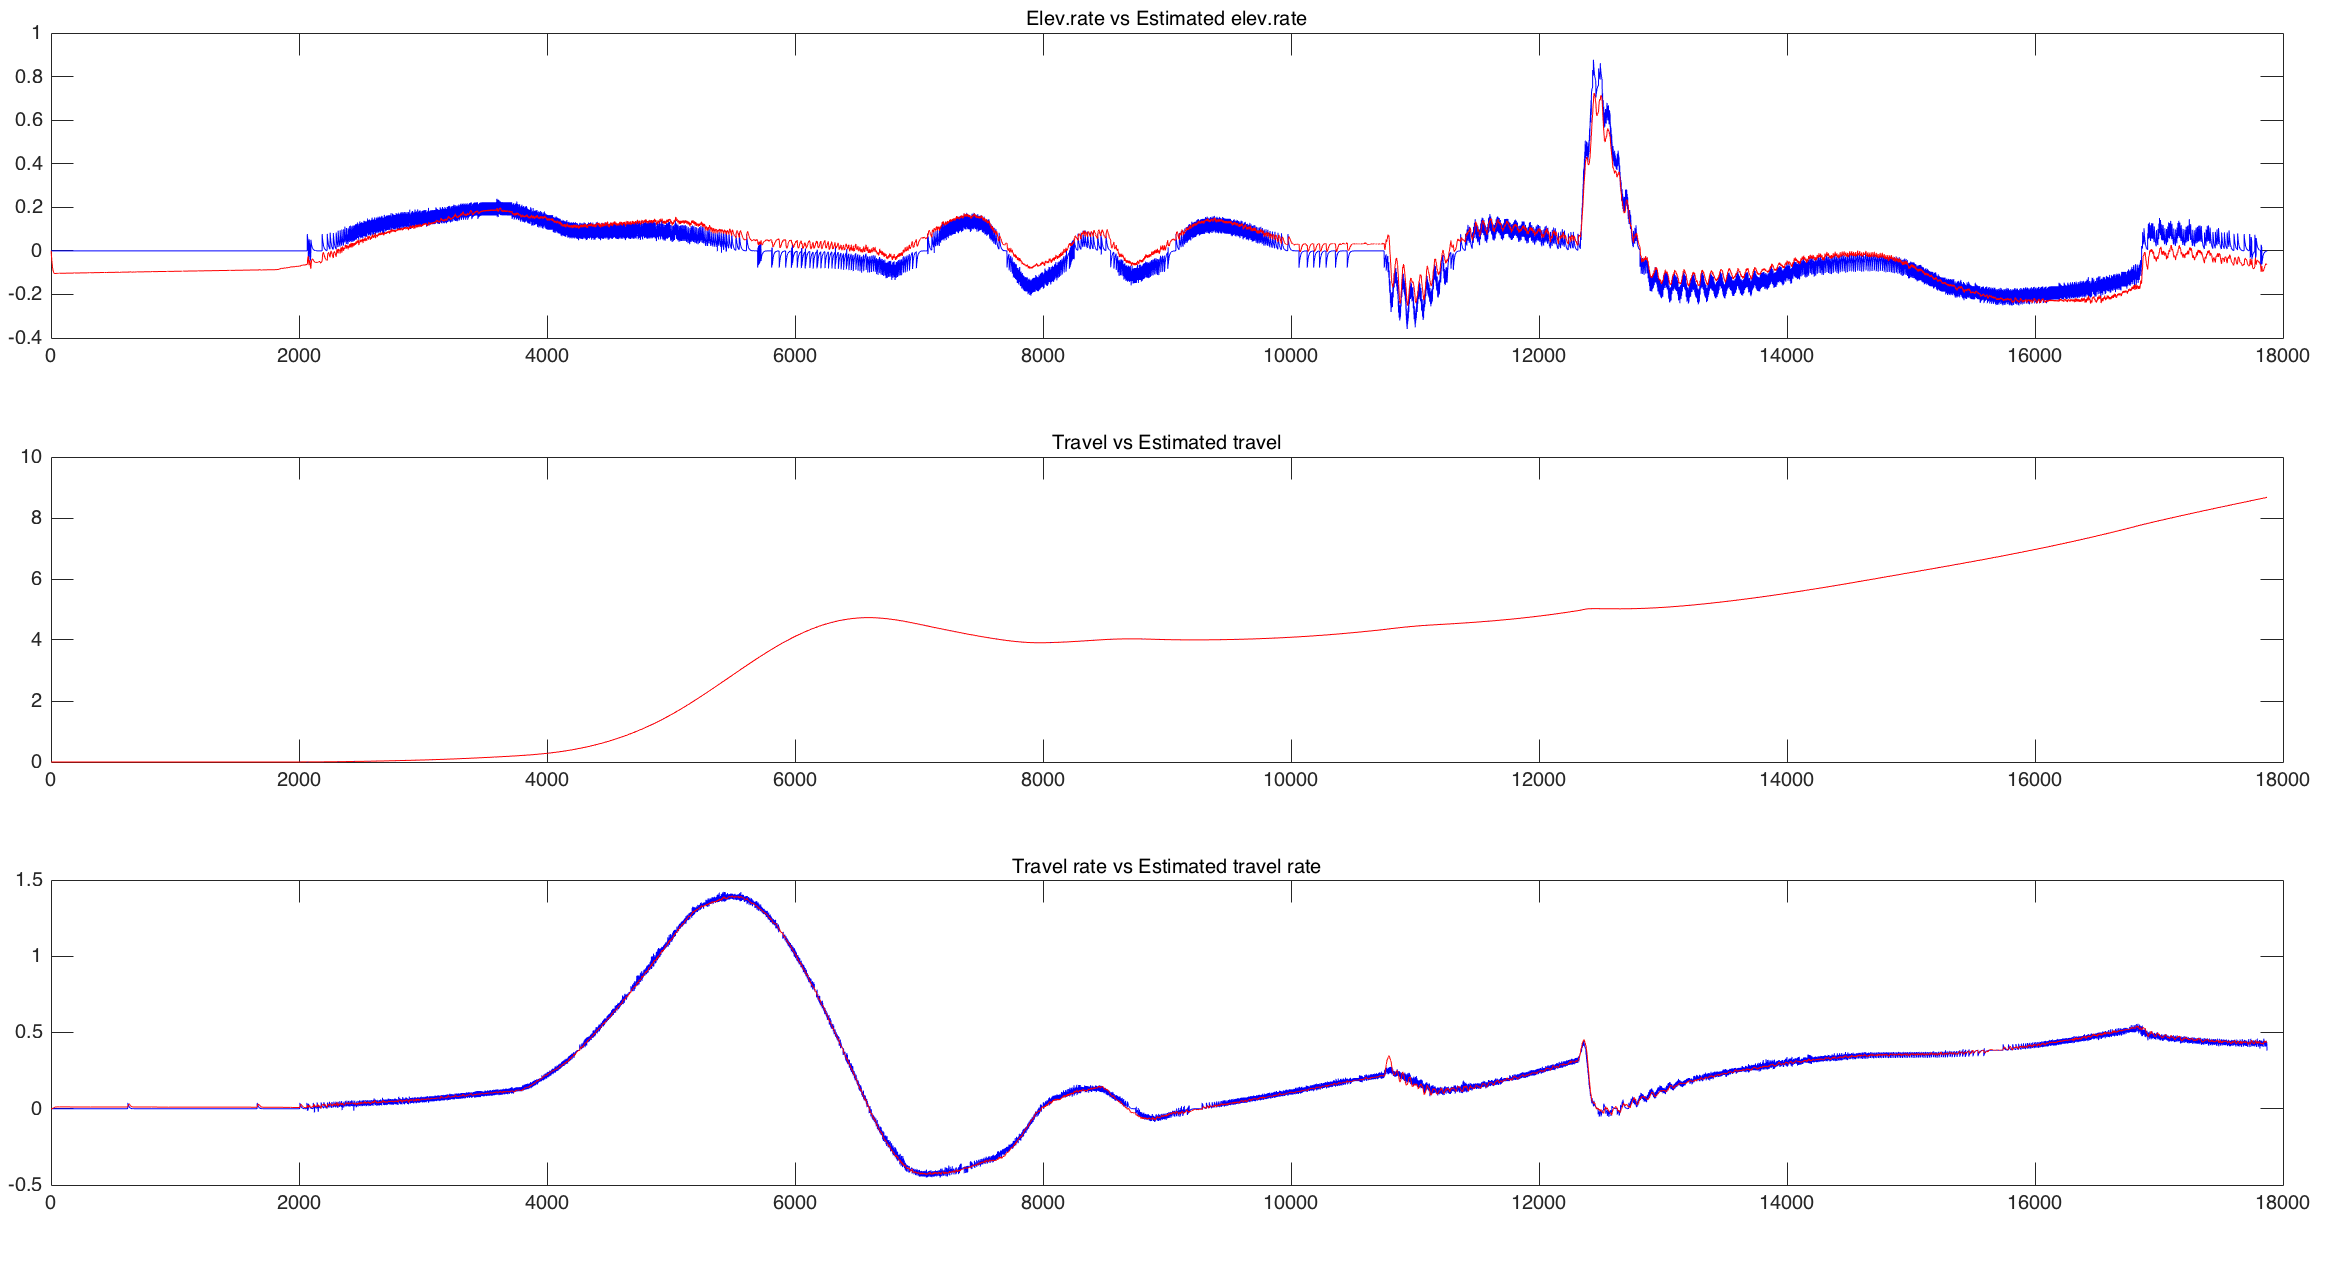
\includegraphics[width=1.0\textwidth]{elevrate_PI.png}
    \caption{Comparison of measured and estimated values of elevation rate, travel and travel rate in the PI-controller (\emph{\color{blue}Blue} = measured value, \emph{\color{red} red} = estimated value)}
    \label{fig:plot4}
\end{figure}

%
\begin{figure}[H]
    \centering
    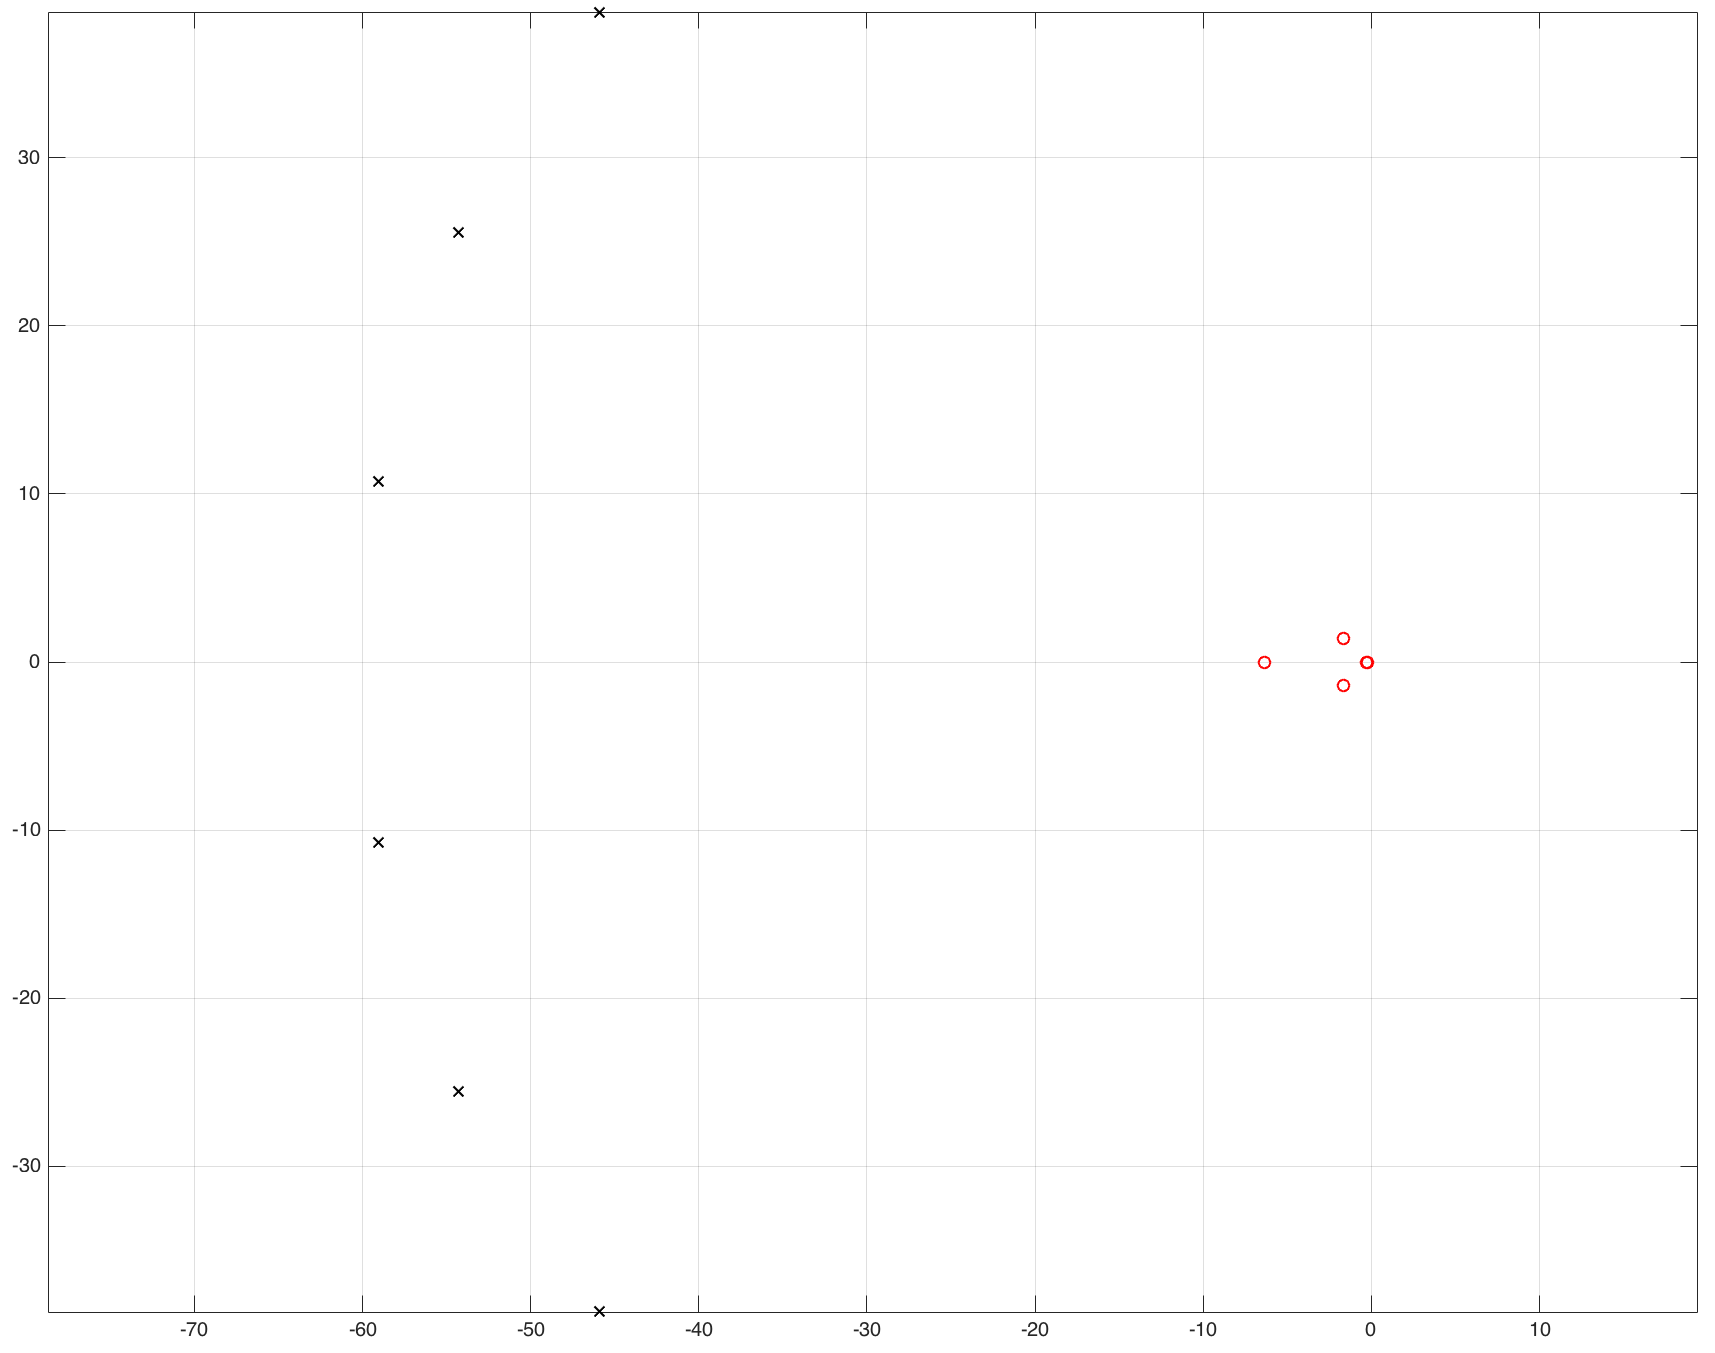
\includegraphics[width=\textwidth]{poleplacement.png}
    \caption{Pole plot of the chosen pole placements (black) and the systems eigenvalues (\emph{\color{red} red}).}
    \label{fig:poles}
\end{figure}
%

\subsection{Observer Using $\tilde{e}$ and $\tilde{\lambda}$}

With the measurable states given in the lab assignment, we alter the output matrices and get the following observability matrices
$$ 
\mathcal{O}_{\tilde{e}\tilde{\lambda}} = 
        \fixTABwidth{T}
        \bracketMatrixstack{
            0&0&1&0&0&0\\
            0&0&0&0&1&0\\
            0&0&0&1&0&0\\
            0&0&0&0&0&1\\
            0&0&0&0&0&0\\
            K_3&0&0&0&0&0\\
            0&0&0&0&0&0\\
            0&K_3&0&0&0&0\\
            0&0&0&0&0&0\\
            0&0&0&0&0&0\\
            0&0&0&0&0&0\\
            0&0&0&0&0&0
        }
    \quad
\mathcal{O}_{\tilde{p}\tilde{\lambda}} = 
        \fixTABwidth{T}
        \bracketMatrixstack{
            1&0&0&0&0&0\\
            0&0&0&0&1&0\\
            0&1&0&0&0&0\\
            0&0&0&0&0&1\\
            0&0&0&0&0&0\\
            K_3&0&0&0&0&0\\
            0&0&0&0&0&0\\
            0&K_3&0&0&0&0\\
            0&0&0&0&0&0\\
            0&0&0&0&0&0\\
            0&0&0&0&0&0\\
            0&0&0&0&0&0
        }
$$
with  $\text{rank}(\mathcal{O}_{\tilde{e}\tilde{\lambda}}) = 6$ and $\text{rank}(\mathcal{O}_{\tilde{p}\tilde{\lambda}}) = 4$. Thus the system is unobservable for 
$\vec{y} = [\tilde{p} \enskip \tilde{e}]^T$, but observable for $\vec{y} = [\tilde{e} \enskip \tilde{\lambda}]^T$. \\

Using $\vec{y} = [\tilde{e} \enskip \tilde{\lambda}]^T$ as the basis for the linear observer gave, using similar controller tuning as previously, very poor performance, especially in controlling the pitch (see \cref{fig:crazyplot1}, \cref{fig:crazyplot2}). This makes sense, as we then are trying to control the helicopter pitch using only the elevation- and travel angles, which is no straight forward task. The controllability matrix suggests it is possible, as the travel is given by the pitch (\ref{eq:6c}), but it requires extensive tuning.
\
%
\begin{figure}[H]
    \centering
    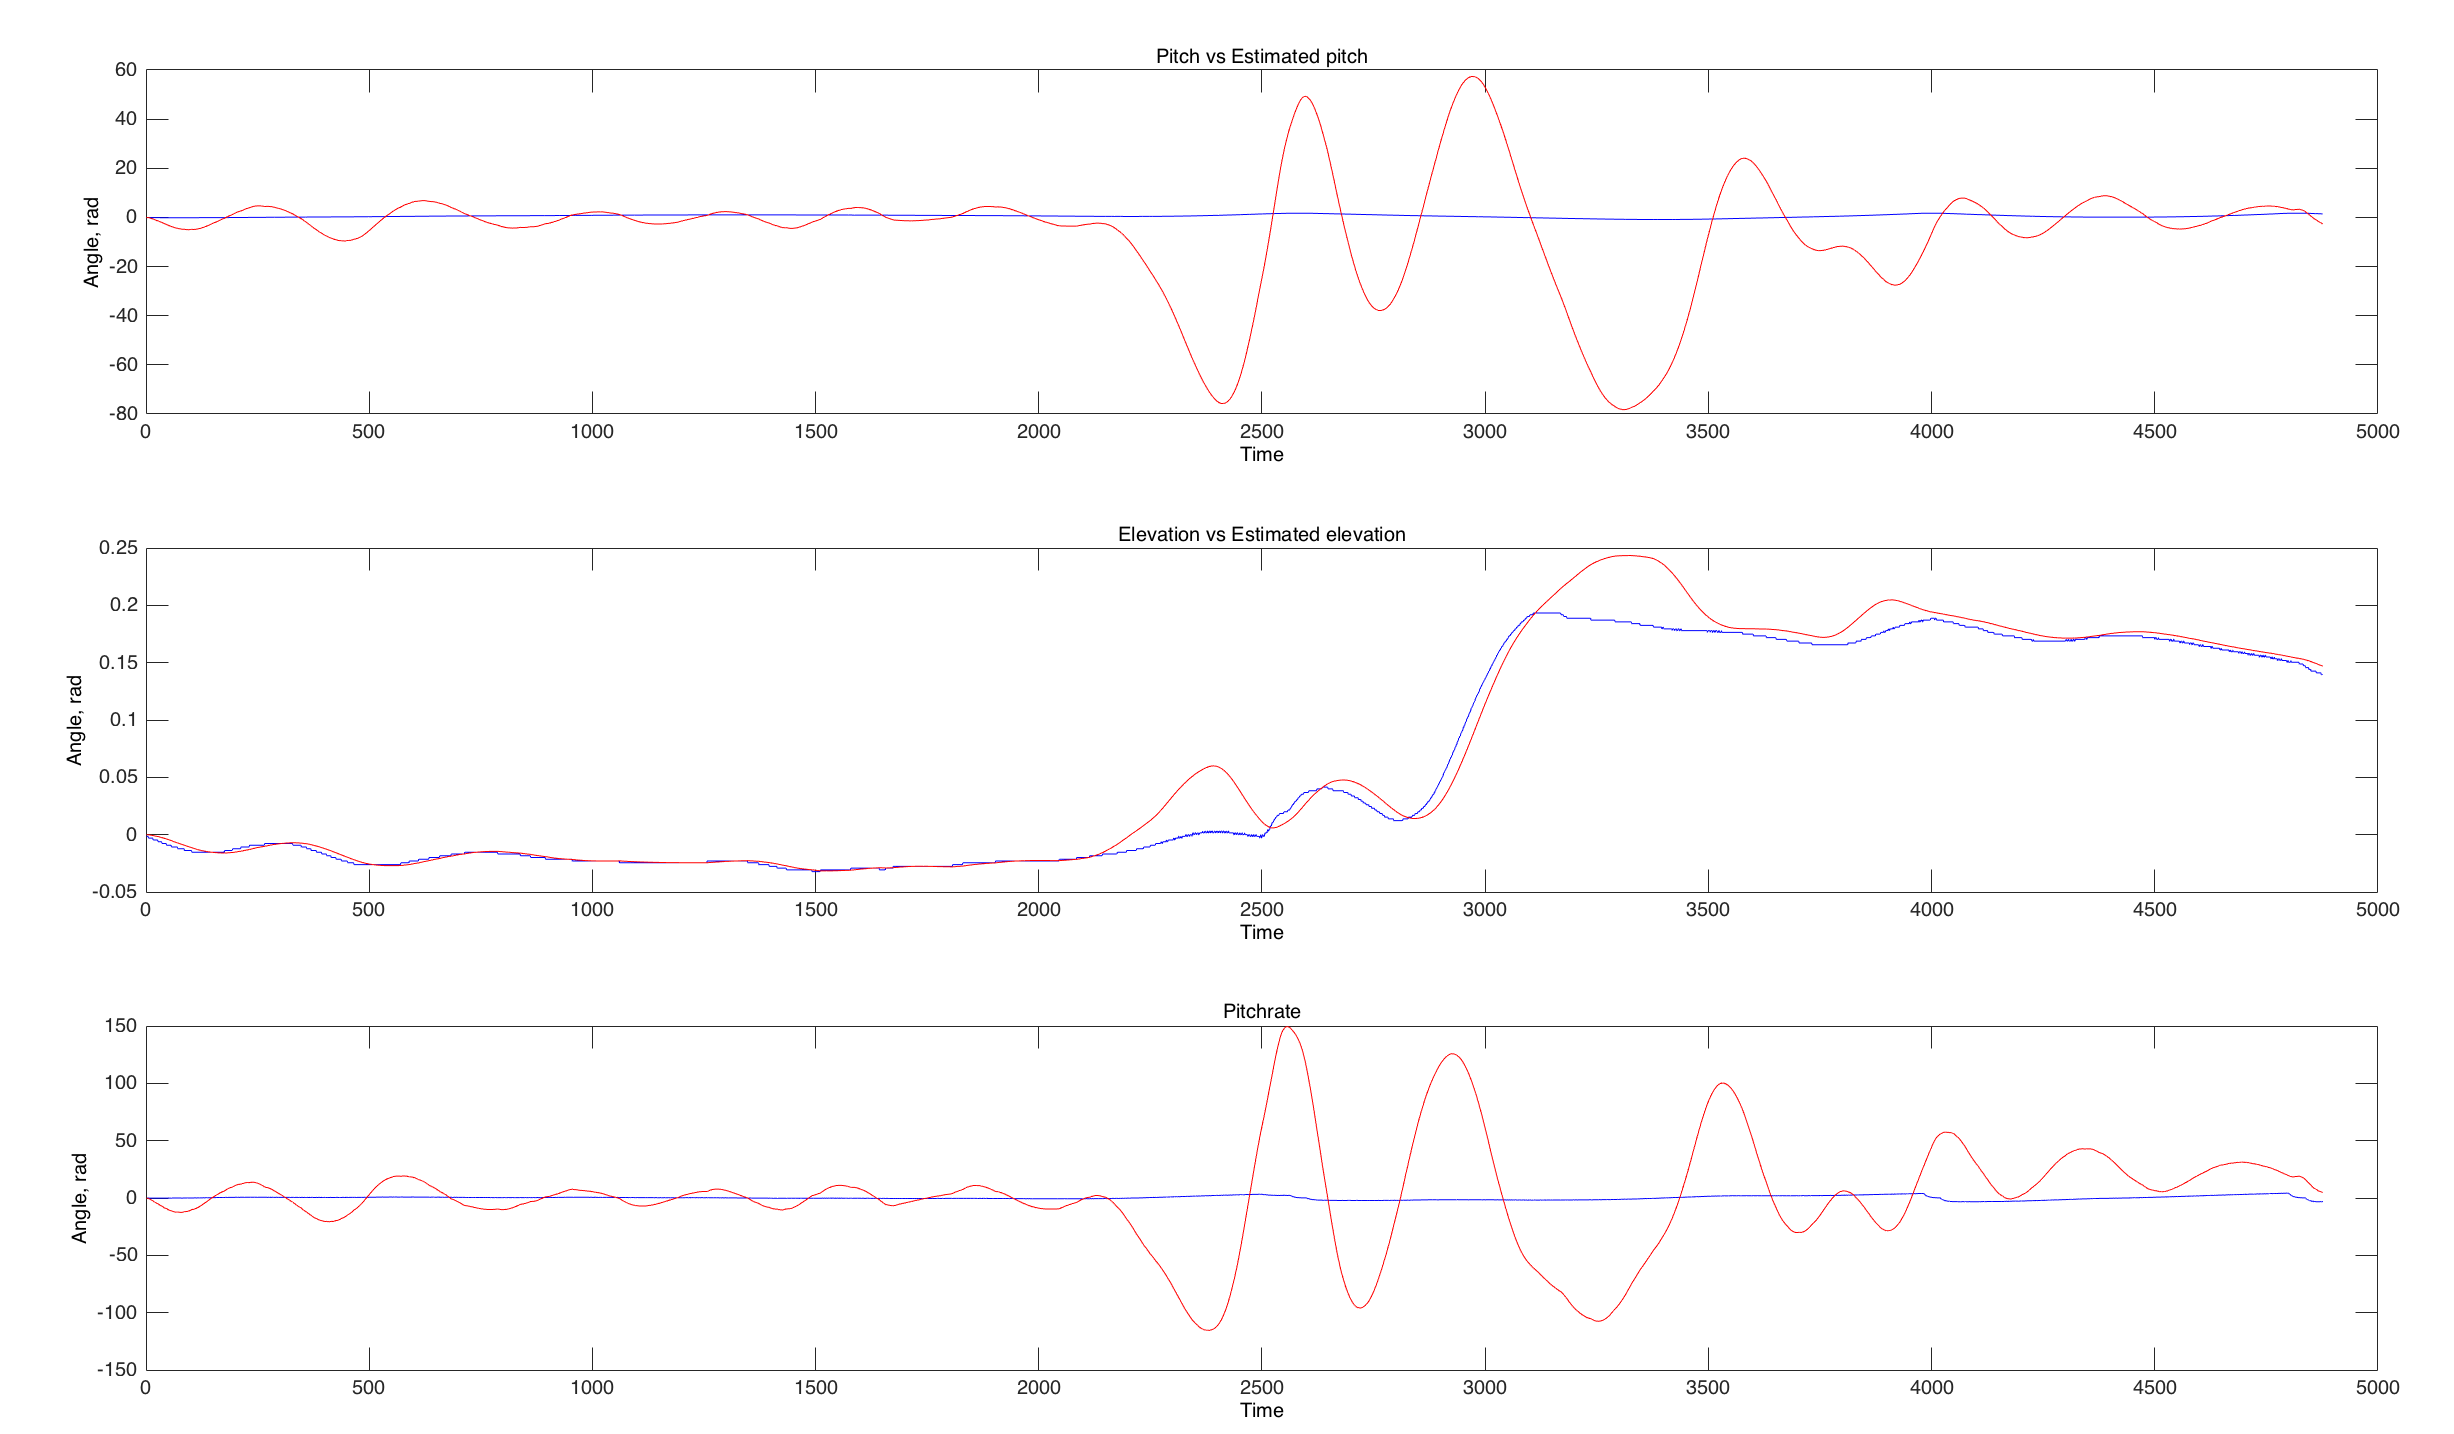
\includegraphics[max size={\textwidth}{\textheight}]{crazyplot2.png}
    \caption{Plot of the true (\emph{\color{blue} blue}) and observed (\emph{\color{red} red}) values of the pitch, elevation and elevation rate.}
    \label{fig:crazyplot1}
\end{figure}
%
\begin{figure}[H]
    \centering
    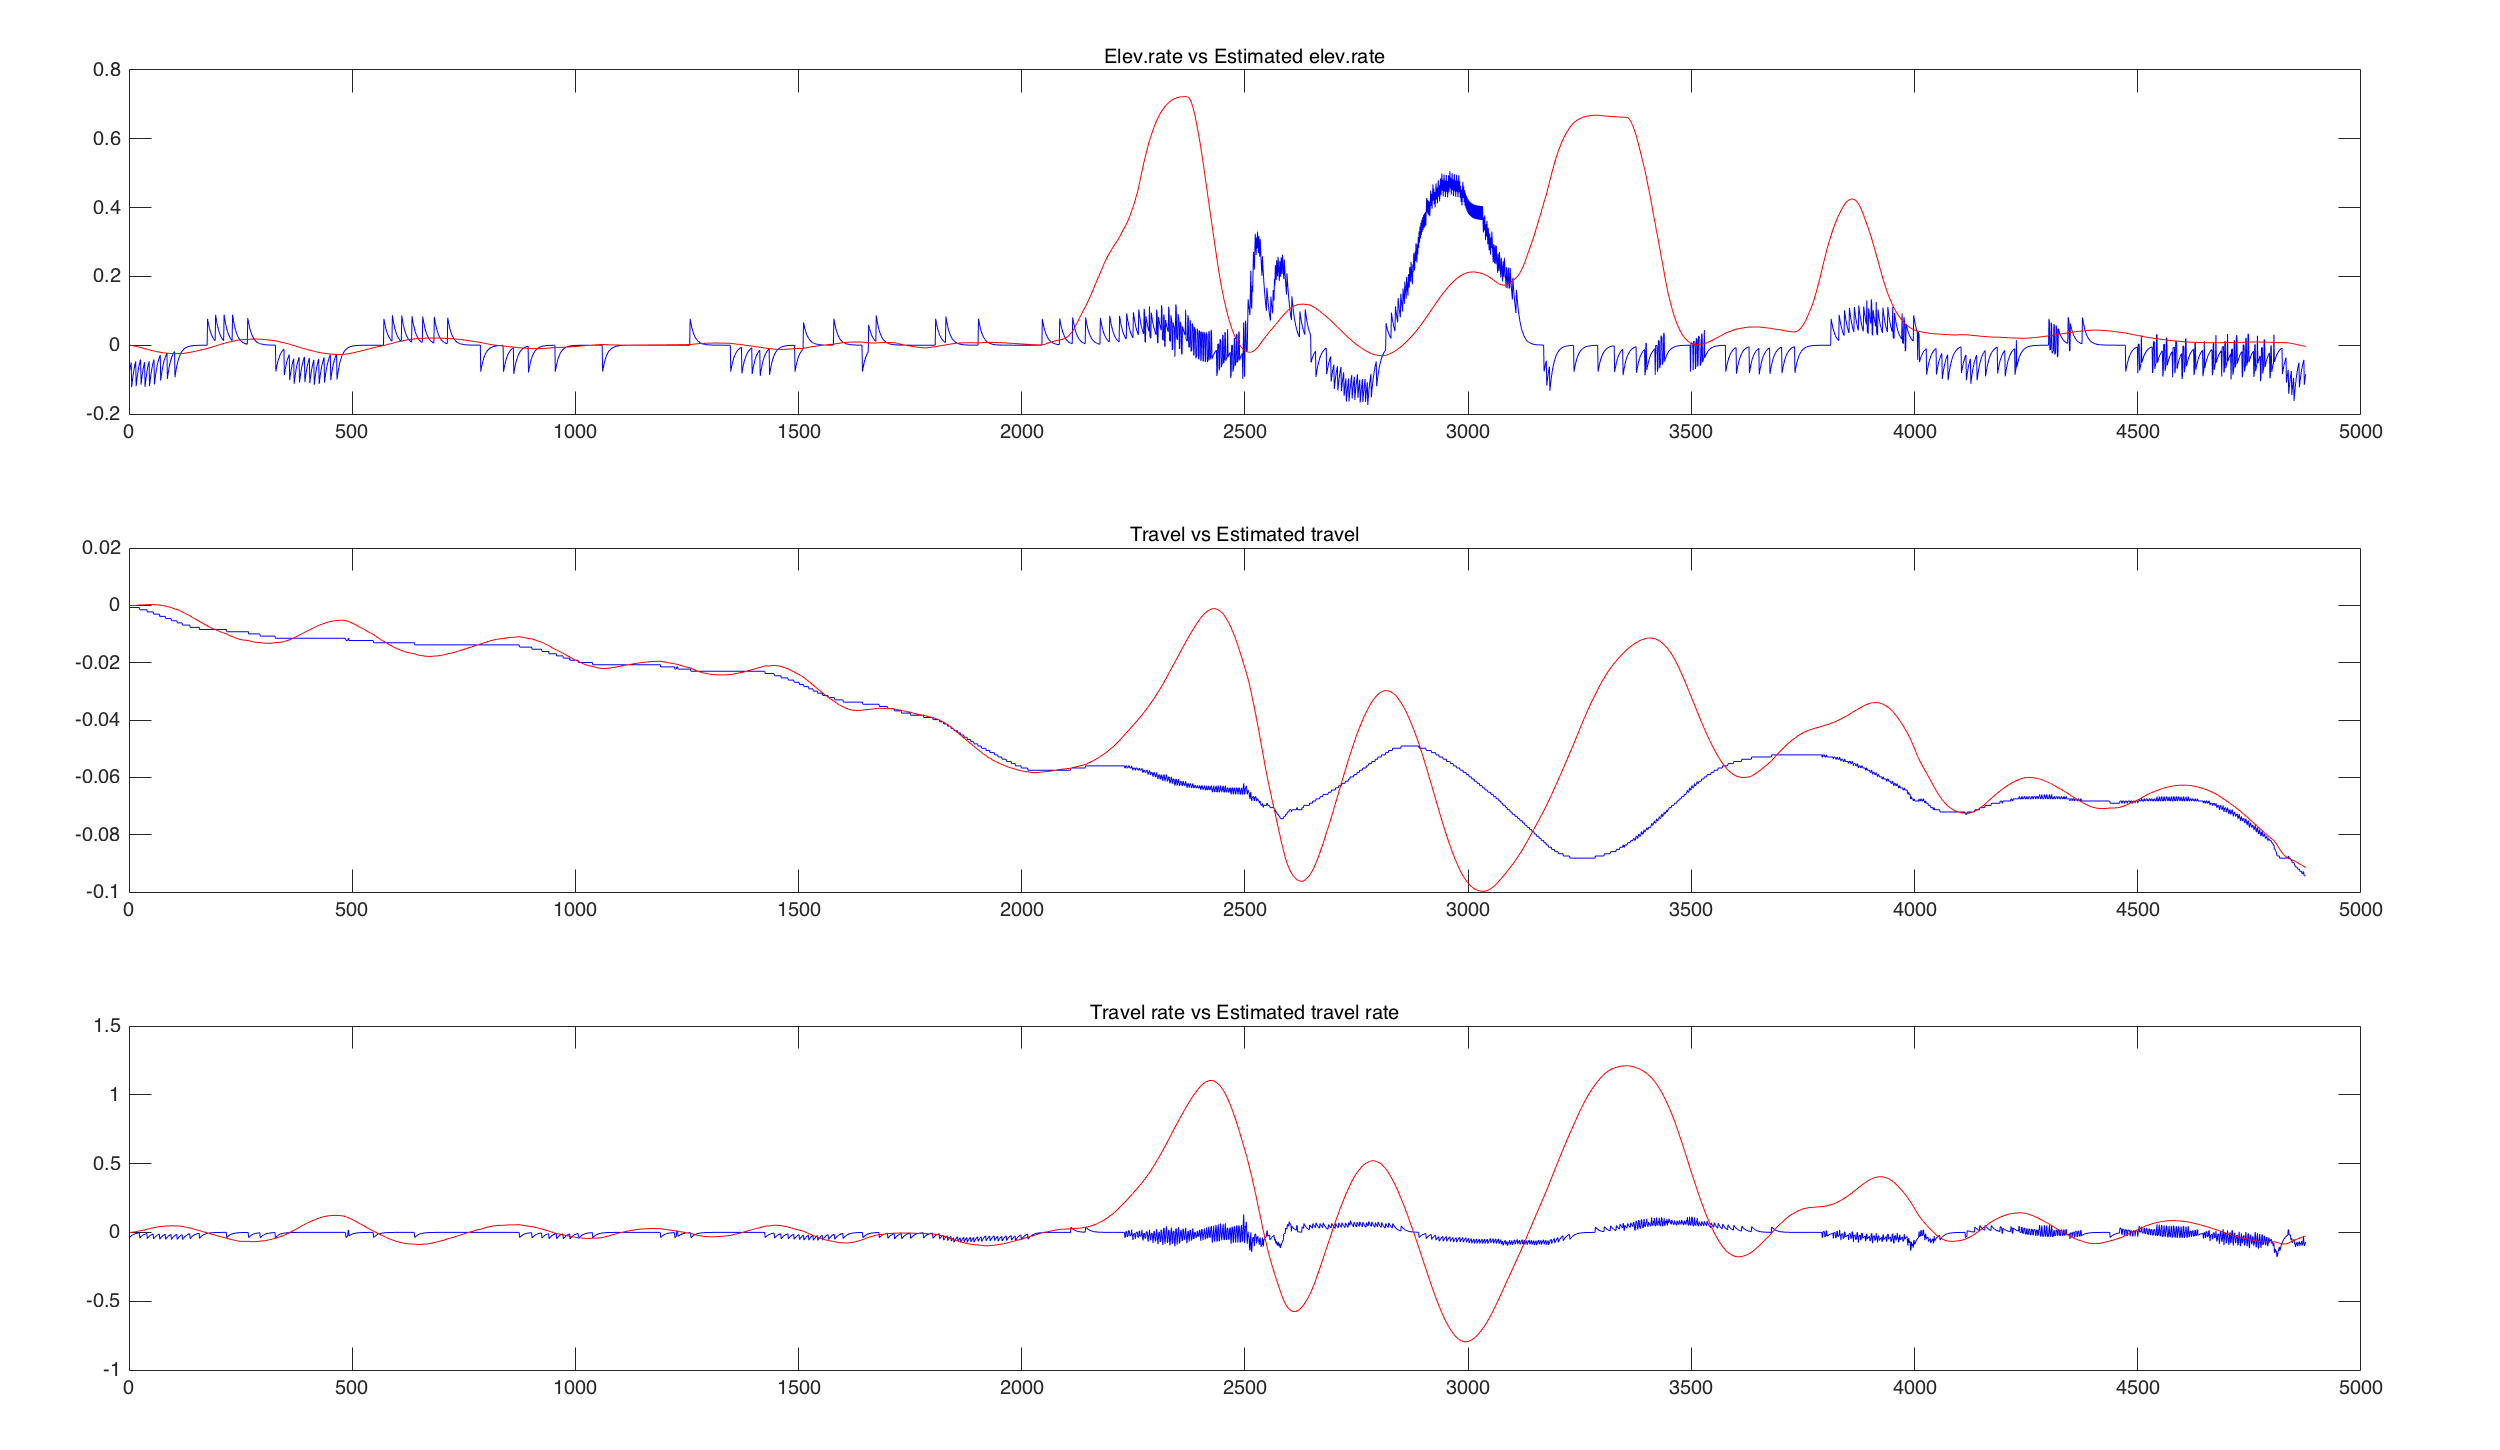
\includegraphics[max size={\textwidth}{\textheight}]{crazyplot1.png}
    \caption{Plot of the true (\emph{\color{blue} blue}) and observed (\emph{\color{red} red}) values of the elevation rate, travel, and travel rate.}
    \label{fig:crazyplot2}
\end{figure}
%